\documentclass[tikz,border=4pt]{standalone}

\usepackage[T1]{fontenc}
\renewcommand{\rmdefault}{ptm}
\usetikzlibrary{arrows.meta,positioning}

\definecolor{Ink}{HTML}{1D303C}
\definecolor{FlowInk}{HTML}{526570}
\definecolor{DataColor}{HTML}{2B6F8A}
\definecolor{RepresentationColor}{HTML}{6B5A94}
\definecolor{ModelColor}{HTML}{B56A24}
\definecolor{OpticsColor}{HTML}{337A58}

\tikzset{
  outer flow/.style={-{Latex[length=1.8mm,width=1.25mm]}, draw=FlowInk, line width=0.8pt},
  representation flow/.style={-{Latex[length=1.55mm,width=1.05mm]}, draw=RepresentationColor, line width=0.75pt},
  model flow/.style={-{Latex[length=1.55mm,width=1.05mm]}, draw=ModelColor, line width=0.75pt},
  optics flow/.style={-{Latex[length=1.55mm,width=1.05mm]}, draw=OpticsColor, line width=0.75pt},
  data group/.style={draw=DataColor!42!white, top color=DataColor!18!white, bottom color=DataColor!5!white,
    rounded corners=4.0pt, line width=0.8pt},
  representation group/.style={draw=RepresentationColor!42!white,
    top color=RepresentationColor!18!white, bottom color=RepresentationColor!5!white,
    rounded corners=4.0pt, line width=0.8pt},
  model group/.style={draw=ModelColor!42!white,
    top color=ModelColor!18!white, bottom color=ModelColor!5!white,
    rounded corners=4.0pt, line width=0.8pt},
  optics group/.style={draw=OpticsColor!42!white,
    top color=OpticsColor!18!white, bottom color=OpticsColor!5!white,
    rounded corners=4.0pt, line width=0.8pt},
  data step/.style={draw=DataColor!30!white, fill=DataColor!5!white,
    rounded corners=2.0pt, line width=0.65pt,
    align=center, text=Ink, font=\rmfamily\fontsize{7.2}{8.3}\selectfont, inner sep=2.2pt},
  representation step/.style={draw=RepresentationColor!30!white, fill=RepresentationColor!5!white,
    rounded corners=2.0pt, line width=0.65pt,
    align=center, text=Ink, font=\rmfamily\fontsize{7.0}{8.0}\selectfont, inner sep=1.8pt},
  model step/.style={draw=ModelColor!30!white, fill=ModelColor!5!white,
    rounded corners=2.0pt, line width=0.65pt,
    align=center, text=Ink, font=\rmfamily\fontsize{7.0}{8.0}\selectfont, inner sep=1.8pt},
  optics step/.style={draw=OpticsColor!30!white, fill=OpticsColor!5!white,
    rounded corners=2.0pt, line width=0.65pt,
    align=center, text=Ink, font=\rmfamily\fontsize{7.0}{8.0}\selectfont, inner sep=2.0pt},
  stage title/.style={font=\rmfamily\bfseries\fontsize{7.5}{8.5}\selectfont,
    align=center},
}
\newcommand{\stagegap}{3.0mm}

\begin{document}
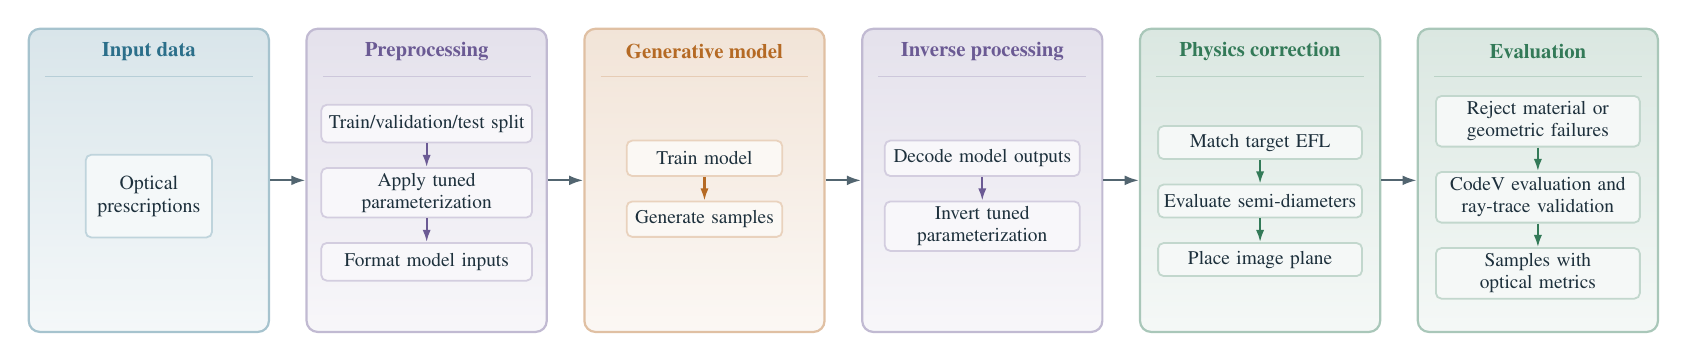
\begin{tikzpicture}[node distance=4.5mm]
  % The established workflow geometry is retained; only its visual treatment changes.
  \node[data group, minimum width=3.05cm, minimum height=3.85cm] (dataStage) {};
  \node[representation group, minimum width=3.05cm, minimum height=3.85cm, right=of dataStage] (pre) {};
  \node[model group, minimum width=3.05cm, minimum height=3.85cm, right=of pre] (model) {};
  \node[representation group, minimum width=3.05cm, minimum height=3.85cm, right=of model] (inverse) {};
  \node[optics group, minimum width=3.05cm, minimum height=3.85cm, right=of inverse] (physics) {};
  \node[optics group, minimum width=3.05cm, minimum height=3.85cm, right=of physics] (codev) {};

  \node[stage title, text=DataColor] at ([yshift=-3.0mm]dataStage.north) {Input data};
  \node[stage title, text=RepresentationColor] at ([yshift=-3.0mm]pre.north) {Preprocessing};
  \node[stage title, text=ModelColor] at ([yshift=-3.0mm]model.north) {Generative model};
  \node[stage title, text=RepresentationColor] at ([yshift=-3.0mm]inverse.north) {Inverse processing};
  \node[stage title, text=OpticsColor] at ([yshift=-3.0mm]physics.north) {Physics correction};
  \node[stage title, text=OpticsColor] at ([yshift=-3.0mm]codev.north) {Evaluation};

  % A quiet header rule echoes the colored title bands in the main publication figure.
  \draw[DataColor!34!white, line width=0.45pt]
    ([xshift=2.2mm,yshift=-6.2mm]dataStage.north west) --
    ([xshift=-2.2mm,yshift=-6.2mm]dataStage.north east);
  \draw[RepresentationColor!34!white, line width=0.45pt]
    ([xshift=2.2mm,yshift=-6.2mm]pre.north west) --
    ([xshift=-2.2mm,yshift=-6.2mm]pre.north east);
  \draw[ModelColor!34!white, line width=0.45pt]
    ([xshift=2.2mm,yshift=-6.2mm]model.north west) --
    ([xshift=-2.2mm,yshift=-6.2mm]model.north east);
  \draw[RepresentationColor!34!white, line width=0.45pt]
    ([xshift=2.2mm,yshift=-6.2mm]inverse.north west) --
    ([xshift=-2.2mm,yshift=-6.2mm]inverse.north east);
  \draw[OpticsColor!34!white, line width=0.45pt]
    ([xshift=2.2mm,yshift=-6.2mm]physics.north west) --
    ([xshift=-2.2mm,yshift=-6.2mm]physics.north east);
  \draw[OpticsColor!34!white, line width=0.45pt]
    ([xshift=2.2mm,yshift=-6.2mm]codev.north west) --
    ([xshift=-2.2mm,yshift=-6.2mm]codev.north east);

  \node[data step, text width=1.45cm, minimum height=1.05cm] (canonical)
    at ([yshift=-2.0mm]dataStage.center) {Optical\\prescriptions};

  \node[representation step, text width=2.55cm, minimum height=0.48cm] (split)
    at ([yshift=7.2mm]pre.center) {Train/validation/test split};
  \node[representation step, text width=2.55cm, minimum height=0.48cm, below=\stagegap of split] (repr)
    {Apply tuned\\parameterization};
  \node[representation step, text width=2.55cm, minimum height=0.48cm, below=\stagegap of repr] (format)
    {Format model inputs};

  \node[model step, text width=1.85cm, minimum height=0.45cm] (train)
    at ([yshift=2.8mm]model.center) {Train model};
  \node[model step, text width=1.85cm, minimum height=0.45cm, below=\stagegap of train] (sample)
    {Generate samples};

  \node[representation step, text width=2.35cm, minimum height=0.45cm] (modelinv)
    at ([yshift=2.8mm]inverse.center) {Decode model outputs};
  \node[representation step, text width=2.35cm, minimum height=0.45cm, below=\stagegap of modelinv] (opticsinv)
    {Invert tuned\\parameterization};

  \node[optics step, text width=2.45cm, minimum height=0.42cm] (eflOp)
    at ([yshift=4.8mm]physics.center) {Match target EFL};
  \node[optics step, text width=2.45cm, minimum height=0.42cm, below=\stagegap of eflOp] (apertureOp)
    {Evaluate semi-diameters};
  \node[optics step, text width=2.45cm, minimum height=0.42cm, below=\stagegap of apertureOp] (imageOp)
    {Place image plane};

  \node[optics step, text width=2.45cm, minimum height=0.42cm] (inputFilterOp)
    at ([yshift=7.5mm]codev.center) {Reject material or\\geometric failures};
  \node[optics step, text width=2.45cm, minimum height=0.42cm, below=\stagegap of inputFilterOp] (codevOp)
    {CodeV evaluation and\\ray-trace validation};
  \node[optics step, text width=2.45cm, minimum height=0.42cm, below=\stagegap of codevOp] (metricsOp)
    {Samples with\\optical metrics};

  \draw[representation flow] (split.south) -- (repr.north);
  \draw[representation flow] (repr.south) -- (format.north);
  \draw[model flow] (train.south) -- (sample.north);
  \draw[representation flow] (modelinv.south) -- (opticsinv.north);
  \draw[optics flow] (eflOp.south) -- (apertureOp.north);
  \draw[optics flow] (apertureOp.south) -- (imageOp.north);
  \draw[optics flow] (inputFilterOp.south) -- (codevOp.north);
  \draw[optics flow] (codevOp.south) -- (metricsOp.north);
  \draw[outer flow] (dataStage.east) -- (pre.west);
  \draw[outer flow] (pre.east) -- (model.west);
  \draw[outer flow] (model.east) -- (inverse.west);
  \draw[outer flow] (inverse.east) -- (physics.west);
  \draw[outer flow] (physics.east) -- (codev.west);
\end{tikzpicture}
\end{document}
